\subsection{Paradigma de Programação}

Um paradigma de programação pode ser definido como um conjunto de princípios que orientam o desenvolvimento de software, e que, consequentemente, geram um software estruturado de uma maneira específica ao paradigma \cite{programmingparadigmsionos}.

Os paradigmas são organizados em categorias, podendo ser vistos como uma hierarquia, assim como mostra a \autoref{fig:hierarquia_paradigmas}:

\begin{figure}[H]
	\centering
	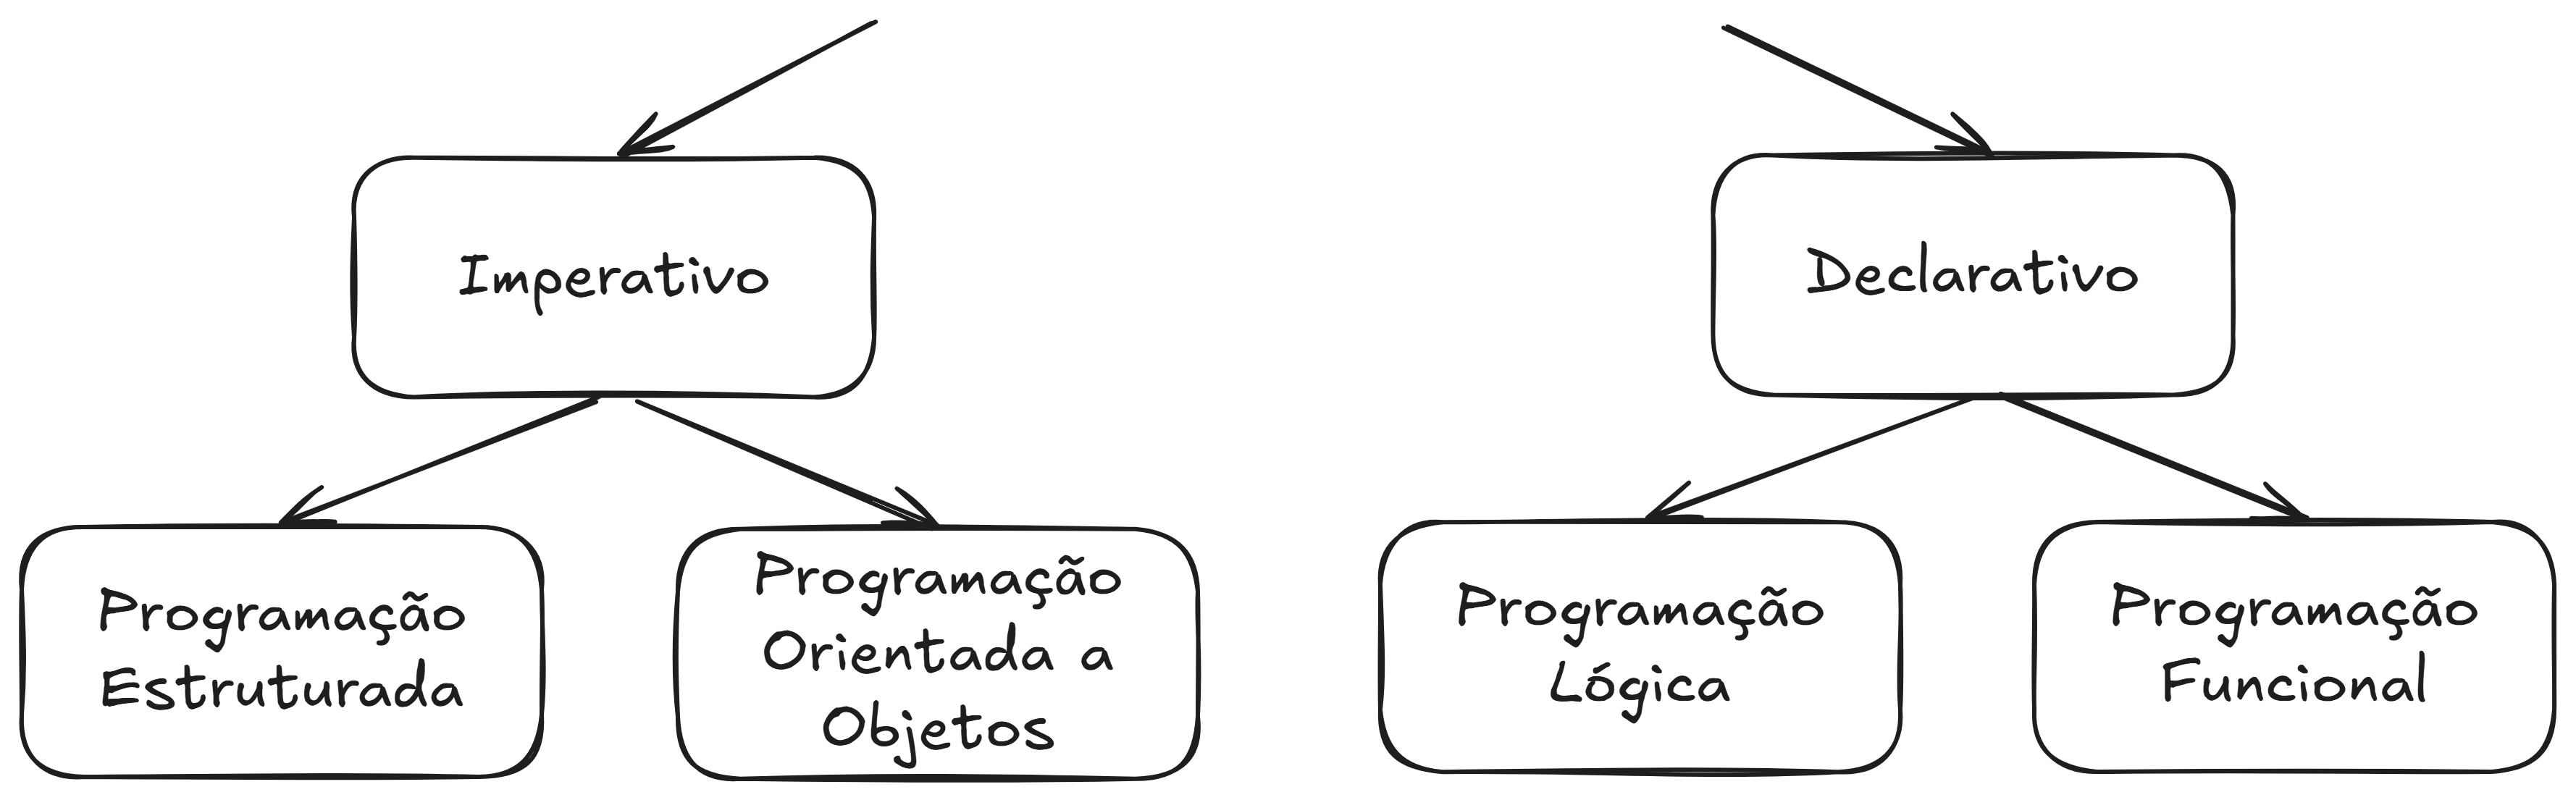
\includegraphics[height=0.17\textheight]{hierarquia_paradigmas}
	\caption{Paradigmas de programação organizados hierarquicamente.}
	\fonte{Adaptado de \citeonline{whatsprogrammingparadigm}.}
	\label{fig:hierarquia_paradigmas}
\end{figure}

Com base na \autoref{fig:hierarquia_paradigmas}, observa-se a relevância dos paradigmas imperativo e declarativo, já que todos os outros paradigmas derivam, em maior ou menor grau, de um desses dois. Por mais que paradigmas mais específicos possam tomar rumos inesperados, eles ainda terão algum grau de herança dos paradigmas imperativo ou declarativo.

Dada a abrangência dos paradigmas imperativo e declarativo, o conhecimento de ambos já se torna suficiente para que o leitor entenda a essência da maioria dos outros paradigmas. Assim, a seguir, eles serão abordados:

\begin{itemize}
	\item Paradigma imperativo: descreve a aplicação em termos de instruções que alteram o estado do programa, linha por linha. O foco está \textit{em como} fazer algo, geralmente oferecendo maior controle e menor abstração. Exemplos de linguagens imperativas incluem C, Java e Python;
	\item Paradigma declarativo: descreve a aplicação em termos de declarações que expressam \textit{o que} o programa deve fazer, e não \textit{em como} fazer. Esta abordagem costuma ser mais abstrata, porém com menos controle. Exemplos de linguagens declarativas incluem SQL, Haskell e Lisp.
\end{itemize}

\subsubsection{O \textit{Entity Component System} pode ser considerado um paradigma?}

O padrão \textit{Entity Component System} (ECS) será extremamente crucial em todas as fases do projeto, por isso, é importante entender em que definição ele se encaixa.

Com base na definição de paradigma dada pelo dicionário Merriam-Webster:

\begin{citacao}
	Uma estrutura filosófica e teórica de uma escola ou disciplina científica dentro da qual teorias, leis e generalizações e os experimentos realizados em apoio a elas são formulados (\citeauthor{merriamwebster}, \citeyear{merriamwebster}, tradução nossa).
\end{citacao}

O autor da biblioteca de ECS Flecs, \citeonline{ecsparadigm}, defende que o ECS não é um paradigma:

\begin{citacao}
	Isso não corresponde exatamente ao ECS. Ter pensamentos profundos sobre o ECS não é o mesmo que ter uma estrutura filosófica. Tutoriais, documentação e postagens em blogs não equivalem a “teorias, leis e generalizações”. É seguro dizer que a base teórica para o ECS é, na melhor das hipóteses, instável (\citeauthor{ecsparadigm}, \citeyear{ecsparadigm}, tradução nossa).
\end{citacao}

Seguindo a conclusão de \citeonline{ecsparadigm}, o ECS não será tratado como um paradigma ao decorrer do projeto, mas sim apenas como um padrão de arquitetura.
